\documentclass[a4paper]{article}
\usepackage{color}              %Farben, f.r \definecolor{}
\usepackage{amssymb}            %Mathematische Symbole
\usepackage{amsthm}             %Besseres \newtheorem
\usepackage{amsmath}           %Mathematische Umgebungen
\usepackage{mathtools}          %\xRightarrow, etc
\usepackage{mathrsfs}           %enthaelt \mathscr
\usepackage{graphicx}
\usepackage{enumerate}          % in-place numerations def.
\usepackage{fullpage}

\usepackage{array}
%\usepackage{multicol}
%\usepackage[notref,notcite]{showkeys}
%\usepackage{algorithm,algorithmic}
\usepackage{color}

\usepackage{graphicx}
\usepackage{xypic}
\entrymodifiers={+!!<0pt,\fontdimen22\textfont2>}
\usepackage[all]{xy}

\usepackage{float}
\usepackage{tikz}
\usepackage{tikz-cd}
\usepackage{tikz,fullpage}
\usetikzlibrary{arrows,%
                petri,%
                topaths}%
\usepackage{tkz-berge}
\usepackage[position=top]{subfig}
\usetikzlibrary{shapes.geometric}
\usetikzlibrary{decorations.markings}

\newtheoremstyle{myremark} % name
    {7pt}                    % Space above
    {7pt}                    % Space below
    {}  	                 % Body font
    {}                           % Indent amount
    {\bf}       	         % Theorem head font
    {.}                          % Punctuation after theorem head
    {.5em}                       % Space after theorem head
    {}  % Theorem head spec (can be left empty, meaning ‘normal’)

\theoremstyle{plain}
\newtheorem{lemma}{Lemma}
\newtheorem{theorem}[lemma]{Theorem}
\newtheorem{fact}[lemma]{Fact}
\newtheorem{definition}[lemma]{Definition}
\newtheorem{corollary}[lemma]{Corollary}
\newtheorem{proposition}[lemma]{Proposition}
\newtheorem{conjecture}[lemma]{Conjecture}
\newtheorem{observation}[lemma]{Observation}
\newtheorem{problem}[lemma]{Problem}
\newtheorem{notation}[lemma]{Notation}
\newtheorem*{claim}{Claim}

\theoremstyle{myremark}
\newtheorem{remark}[lemma]{Remark}
\newtheorem{example}[lemma]{Example}
\newtheorem{exercise}[lemma]{Exercise}
\newtheorem{algorithm}[lemma]{Algorithm}
\newtheorem{application}[lemma]{Application}
\newtheorem*{goal}{Goal}

\newcommand{\RR}{\mathbb{R}}
\newcommand{\vol}{\mathrm{Vol}}

%%%%%% EDIT HERE: %%%%%%%%%%%
\newcommand{\LECTURENUMBER}{12}
\newcommand{\LECTURETITLE}{Coloring Euclidean spaces. Unit distance graphs.}
\newcommand{\LECTURESCRIBE}{M.A.}

%% Dokument Beginn %%%%%%%%%%%%%%%%%%%%%%%%%%%%%%%%%%%%%%%%%%%%%%%%%%%%%%%%
\begin{document}
\thispagestyle{empty}

\begin{center}
	{\Large\bf Graph coloring}\\
	{\bf Lecture notes, vol. \LECTURENUMBER \\ 
	\LECTURETITLE}\\
\end{center}
Lecturer: Michal Adamaszek \hfill Scribe: \LECTURESCRIBE
\begin{center}
\line(1,0){450}
\end{center}

%%%%%%% EDIT ALSO BELOW: %%%%%%%%%%%%%%%%
Last time we defined $\chi(\RR^d)$ as the smallest number of colors required to color $\RR^d$ so that any two points in distance $1$ have different colors. For any subset $X\subseteq \RR^d$ we defined the (possibly infinite) graph $U_X$ with vertex set $X$ and with edges between any two points at distance exactly $1$. Of course $\chi(\RR^d)=\chi(U_{\RR^d})$. We also showed $\chi(\RR^2)\leq 9$.

\begin{proposition}
$\chi(\RR^2)\leq 7.$
\end{proposition}
\begin{proof}
Consider a covering of $\RR^2$ with squares of diagonal $1$ (that is, of side $1/\sqrt{2}$):

\begin{center}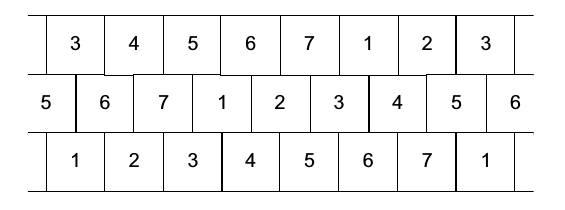
\includegraphics[scale=0.4]{mf9.png}\end{center}

Use the colors as indicated, remembering to color the interior of the square, its top-right corner, the top edge without the top-left corner and the right edge without the bottom-right corner.
\end{proof}

\begin{remark}
Another coloring uses a covering by hexagons. Each small hexagon should have diameter $0.99$:
\begin{center}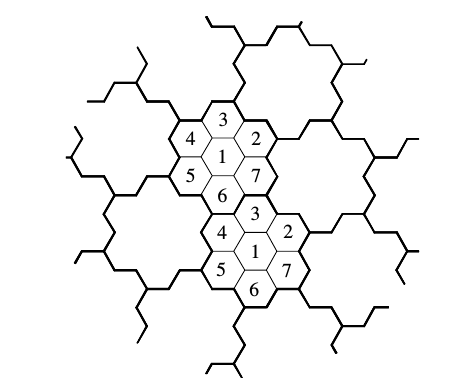
\includegraphics[scale=0.4]{mf5.png}\end{center}
\end{remark}


\begin{proposition}
$\chi(\RR^2)\geq 4.$
\end{proposition}
\begin{proof}
Suppose, on the contrary, that $c:\RR^2\to\{1,2,3\}$ is a coloring of $U_{\RR^2}$ with $3$ colors. I claim that 
$$d(x,y)=\sqrt{3} \implies c(x)=c(y).$$
Indeed, if $d(x,y)=\sqrt{3}$ then there are points $z,t$ with $d(x,z)=d(y,z)=d(x,t)=d(y,t)=d(z,t)=1$, because $x,y$ are the ``opposite'' vertices of two equilateral triangles joined at one base. Since $c(x),c(z),c(t)$ are all different and so are $c(y),c(z),c(t)$, we conclude $c(x)=c(y)$.

It means that for any $x\in\RR^2$, all points on the circle centered at $x$ of radius $\sqrt{3}$ have the same color. But on that circle we can find two points in distance $1$, contradiction.
\end{proof}

\begin{remark}
The proof above can be turned into a construction of a finite subgraph $H$ of $U_{\RR^2}$ with $\chi(H)=4$. It is called the Moser graph, left. Another graph with this property is the Golomb graph, right.
\begin{center}
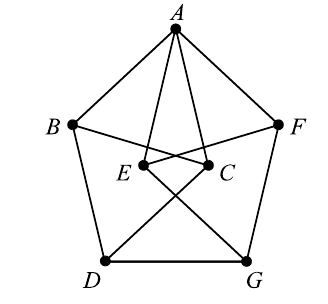
\includegraphics[scale=0.4]{mf6.png}
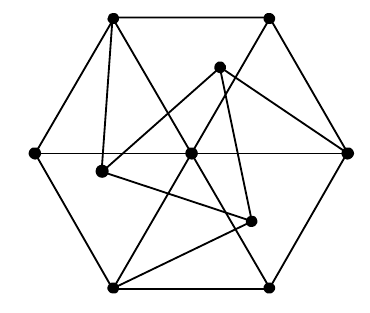
\includegraphics[scale=0.4]{mf7.png}
\end{center}
\end{remark}
\begin{remark}
The bounds $4\leq\chi(\RR^2)\leq 7$ are all that we know in general about $\chi(\RR^2)$.
\end{remark}


We can now move on to higher dimensions, where the gaps in our knowledge are even bigger. For example, it is only known that
$$6\leq\chi(\RR^3)\leq 15.$$
However, the rate of growth of $\chi(\RR^d)$ as $d\to\infty$ is generally understood to be exponential.

\begin{theorem}
There are constants $1<c_1<c_2$ such that for all $d$:
$$c_1^d\leq \chi(\RR^d)\leq c_2^d.$$
\end{theorem}
The current best are $c_1\approx 1.23$ and $c_2=3+\varepsilon$. We are not going to prove the theorem with the optimal constants, but we are going to show some weaker exponential upper and lower bounds. There will be some especially nice mathematics involved in the lower bounds, in particular!

We start with an upper bound.

\begin{theorem}
For sufficiently large $d$ we have $\chi(\RR^d)\leq 14^d$.
\end{theorem}
\begin{proof}
We will tile $\RR^d$ with small cubes, and color each cube with one color, similarly to the $3\times 3$ strategy used to show $\chi(\RR^2)\leq 9$. As we saw in the exercises, repetitive coloring may not work for $d\geq 4$. Instead, we will color the small cubes greedily.

For simplicity, suppose first that $d=2k$. We need two prerequisites: the formula for the volume of the $d$-dimensional ball $B_d(x,r)$ with center $x$ and radius $r$ for $d=2k$ is
$$\vol(B_d(x,r)) = \frac{\pi^k}{k!}r^{2k}.$$
We will also need the inequality $k!\geq(k/e)^k$, or equivalently $k^k/k!\leq e^k$.

Divide $\RR^d$ into ``small cubes'' of size
$$0.99\frac{1}{\sqrt{d}}\times 0.99\frac{1}{\sqrt{d}}\times\cdots\times 0.99\frac{1}{\sqrt{d}}.$$
Each cube has diameter (main diagonal) $0.99<1$ and volume $0.99^dd^{-d/2}=0.99^{2k}(2k)^{-k}$. Denote any such small cube by $C$.

Now we ask: how many small cubes are completely contained in any  ball $B_d(x,3)$ of radius $3$? Comparing volumes gives that this number is \emph{at most}
\begin{align*}
\frac{\vol(B_d(x,3))}{\vol(C)} = \frac{3^{2k}\pi^k(2k)^k}{k!0.99^{2k}}=\frac{k^k}{k!}\cdot(\frac{18\pi}{0.99^2})^k\leq (\frac{18\pi e}{0.99^2})^k<163^k<13^d.
\end{align*}

Now order the (countably many) small cubes into a sequence $C_1,C_2,\ldots$ and let $x_i$ be the center of $C_i$. We color each $C_i$ according to the greedy rule: choose any color that is not used for cubes $C_j$, $j<i$ such that $C_j\subseteq B_d(x_i,3)$. By the previous observation there are at most $13^d-1$ cubes $C_j$ we have to consider, and there always is a spare color so that the greedy algorithm will do with at most $13^d$ colors. (It does not matter which color we use on points common to more than one cube, for example we can color closed cubes and repaint anything that is already colored).

Now, two points inside one small cube are in distance at most $0.99<1$. Consider two points $x,y$ with $d(x,y)=1$ and let $x\in C_i$, $y\in C_j$, with $i>j$. By the triangle inequality we have that for any point $z\in C_j$ 
$$d(x_i,z)\leq d(x_i,x)+d(x,y)+d(y,z)\leq 0.99+1+0.99<3$$
so $C_j\subseteq B_d(x_i,3)$. It means that the greedy algorithm used different colors for $x\in C_i$ and $y\in C_j$, and so we showed $\chi(\RR^d)\leq 13^d$.

If $d$ is odd and large enough then $\chi(\RR^d)\leq \chi(\RR^{d+1})\leq 13^{d+1}<14^d$ by what we already showed.
\end{proof}

We can now move on to lower bounds. Clearly, we have $\chi(\RR^d)\geq \omega(U_{\RR^d})=d+1$, but that is far from exponential. 

\begin{definition}
We say a finite graph $G$ is a \emph{unit distance graph in $\RR^d$} if there is a set $X\subseteq \RR^d$  with $|X|=|V(G)|$ for which $G$ is isomorphic to $U_X$.
\end{definition}

\begin{lemma}
If $G$ is a unit distance graph in $\RR^d$ then $\chi(\RR^d)\geq \chi(G)$.
\end{lemma}
\begin{proof} For $X$ as in the definition, we have
$U_X\subseteq U_{\RR^d}$, so $\chi(\RR^d)=\chi(U_{\RR^d})\geq \chi(U_X)=\chi(G)$.
\end{proof}

\begin{example}
\begin{itemize}
\item The Moser and Golomb graphs are unit distance graphs in $\RR^2$.
\item The $d$-cube graph $Q_d$ is a unit distance graph in $\RR^d$. However, $\chi(Q_d)=2$, so it does not provide useful lower bounds.
\item Take the vertices of the $3$-cube $Q_3$, but this time instead of the edges of the cube, take a graph formed by all the diagonals of the faces of the cube. There are $12$ of them, each of length $\sqrt{2}$, so they form a unit distance graph in $\RR^3$ (after rescaling by $1/\sqrt{2}$). We see that this graph  is isomorphic to $K_4\sqcup K_4$, so it yields $\chi(\RR^3)\geq 4$. We knew that already, but it is better than with the standard cube.
\end{itemize}
\end{example}

\begin{definition}
For $1\leq u\leq d$ let $Q_d(u)$ be the graph whose vertices are all binary sequences of length $d$:
$$V(Q_d(u))=\{(x_1,\ldots,x_d)~:~x_i\in\{0,1\}\}$$
and two sequences are adjacent in $Q_d(u)$ if and only if they differ in exactly $u$ positions.
\end{definition}
\begin{example}
\begin{itemize}
\item $Q_d(1)=Q_d$.
\item $Q_3(2)=K_4\sqcup K_4$ is the graph from the previous example.
\item $Q_d(d)$ is a disjoint union of $2^{d-1}$ copies of $K_2$.
\end{itemize}
\end{example}

\begin{lemma}
Each $Q_d(u)$ is a unit distance graph in $\RR^d$.
\end{lemma}
\begin{proof}
Every vertex of $Q_d(u)$ can be treated as a point in $\RR^d$ with the same coordinates. If $(x_1,\ldots,x_d)$ and $(y_1,\ldots,y_d)$ are seqnences of $0$s and $1$s which differ in exactly $u$ positions, then their Euclidean distance is $\sqrt{u}$. 
\end{proof}

\begin{remark}
The graphs $Q_d(u)$ provide good lower bounds for $\chi(\RR^d)$ for small $d$ (as we will see experimentally in the exercises). They also provide exponential lower bounds for large $d$ (next lecture).
\end{remark}

\begin{remark}
Figures taken from the book \emph{The Mathematical Coloring Book: Mathematics of Coloring and the Colorful Life of its Creators} by Alexander Soifer.	
\end{remark}
\end{document}




